\documentclass[handout]{beamer}
\usepackage{bm}
\usepackage{listings}
\usepackage{algorithmic}
\usepackage{verbatim}
\usepackage{rotating}
\usepackage{multirow}
\lstloadlanguages{R}
\lstset{ language=R, basicstyle=\scriptsize\ttfamily, commentstyle=\ttfamily\color{gray}, numbers=left, numberstyle=\ttfamily\color{gray}\footnotesize, stepnumber=1, numbersep=5pt, backgroundcolor=\color{white}, showspaces=false, showstringspaces=false, showtabs=false, frame=single, tabsize=2, captionpos=b, breaklines=true, breakatwhitespace=false, escapeinside={}, keywordstyle={}, morekeywords={} }\renewcommand{\P}{\mathcal{P}}
\newcommand{\bt}{\pmb{\theta}}
\newcommand{\bG}{\pmb{\Gamma}}
\newcommand{\p}{\pause}
\newcommand{\pitem}{\pause \item}
\newcommand{\N}{\mathcal{N}}
\newcommand{\Y}{\bm{\mathcal{Y}}}
\newcommand{\bh}{\bm{h}} 
\DeclareMathOperator*{\argmax}{arg\,max}

\usefonttheme{serif}

\newenvironment{changemargin}[2]{%
  \begin{list}{}{%
    \setlength{\topsep}{0pt}%
    \setlength{\leftmargin}{#1}%
    \setlength{\rightmargin}{#2}%
    \setlength{\listparindent}{\parindent}%
    \setlength{\itemindent}{\parindent}%
    \setlength{\parsep}{\parskip}%
  }%
  \item[]}{\end{list}} 

%
\title{Inferential Network Analysis with \\ Exponential Random Graph Models}
%
\definecolor{umassred}{HTML}{001769}
\setbeamercolor{structure}{fg=umassred} 
\author{Bruce A. Desmarais}

%\affil[1]{University of Massachusetts Amherst}
%\affil[2]{University of Connecticut}


\begin{document}
%\date{November 16, 2012}

\begin{frame}
  \titlepage
\end{frame}


% Introducing Network Analysis

\begin{frame}
\frametitle{What does it mean to model the network?}
\Large
Construct a probability distribution that \\~\\ accurately approximates the network
\end{frame}


\begin{frame}
\frametitle{Why build models?}

\begin{itemize}
\item {\Large Test hypotheses}\\
{\bf Example:} Does the cosponsorship network exhibit reciprocity? \\~\\
\item {\Large Simulation for theoretical exploration}
{\bf Example:} How should seats be assigned in a classroom to encourage cross-racial friendships? \\~\\
\item {\Large Tie prediction} \\
{\bf Example:} Will Canada attack next year?

\end{itemize}
\end{frame}



% Presenting Interdependence Problem
\begin{frame}
\frametitle{Modeling Interdependence}

{\bf Two Classes of Questions:} Covariate and Interdependence
\begin{enumerate}
\item Covariate
\begin{itemize}
\item Do legislators in the same political party collaborate more frequently than those in opposite parties?
\item Do states with democratic governments have more alliances than those with autocratic regimes?
\end{itemize}
\item Interdependence
\begin{itemize}
\item Are two states at war with the same third state less likely to be at war with each other?
\item Are there popularity effects in the choice of co-authors?
\end{itemize}
\end{enumerate}
{\bf ERGM:} integrate effects for any forms of (1) and (2) into a unified model of a network.
\begin{center}
\begin{changemargin}{-.5cm}{-1cm}
\includegraphics[scale=.25]{allTriads.jpg}
\end{changemargin}
\end{center}
\end{frame}





% A crash course in the likelihood framework 
\begin{frame}
\frametitle{Parametric Probabilistic Modeling \\ and the Likelihood Framework of Inference}
We observe $x$, a draw of a random variable $X$.. $$ X\sim f(X,\bt)$$
$f$ is a family of probability distributions and $\bt$ is unknown.
\\ $X$ could be
\begin{itemize}
\item The dependent variable in a regression model
\item An adjacency matrix
\item The text in a document
\end{itemize}
$$\hat{\bt}_{MLE} = \argmax_{\bt}\left[f(x,\bt)\right] $$
\begin{enumerate}
\item In many cases, $\hat{\bt}_{MLE}$ is asymptotically normally distributed
\item If $f$ is exponential family, $\ln\left[f(x,\bt)\right]$ globally concave in $\bt$
\end{enumerate}

\end{frame}


% Presentation of ERGM Models

\frame{
\frametitle{The Exponential Random Graph Model (ERGM)}\vspace{0.5cm}

The probability (likelihood function) of observing network $N$ is:
\[
\mathcal{P}(N, \bt) = \frac{\exp \{ \bt' \bh(N)  \}}{\sum_{N^* \in \mathcal{N}} \exp \{\bt ' \bh(N^*)  \}}
\]
Decomposition:
\[
\underbrace{\bh(N)}_{Net\hspace{3pt} Stats} \qquad \underbrace{\bt}_{Effects} \qquad \underbrace{\exp \{\bt' \bh(N) \}}_{+ \hspace{3pt} Weight} \qquad \underbrace{\sum_{N^* \in \mathcal{N}} \exp \{\bt ' \bh(N^*)  \}}_{Normalizer}
\]

Flexible: $\bh$ can capture virtually any form of interdependence among the edges $+$ covariates\\
\vspace{0.5cm}
Normalizing constant can make estimation difficult
}




\begin{frame}
\frametitle{Definining $\bh$}

\Large

How would we measure {\bf reciprocity}?
\\~\\
A statistic we would expect to be high if ties were reciprocated a lot and low if they were not reciprocated.


\end{frame}



%%% Specification Examples

\begin{frame}
\frametitle{Unpacking $\bh$}
\begin{itemize}
\item Dyadic Covariate $$ h_D(N,X) = \sum_{ij} N_{ij}X_{ij} $$
\item Sender Covariate $$ h_{VS}(N,VS) = \sum_{i}VS_i\sum_{j \neq i} N_{ij} $$
\item Receiver Covariate $$ h_{VR}(N,VR) = \sum_{i}VR_i\sum_{j \neq i} N_{ji} $$
\item Reciprocity 
\[
h_R(N)=\sum_{i < j }N_{ij}N_{ji}
\]
\begin{center}
\includegraphics[height=1.5cm]{reciprocity.jpg}
\end{center}
\end{itemize}
\end{frame}

\begin{frame}
\frametitle{Unpacking $\bh$}
\begin{itemize}
\item Popularity
\[
h_P(N) = \sum_{i,j,k} N_{ji}N_{ki}+N_{kj}N_{ij}+N_{ik}N_{jk}
\]
\item Sociality
\[
h_S(N) = \sum_{i,j,k} N_{ij}N_{ik}+N_{jk}N_{ji}+N_{ki}N_{kj}
\]
\begin{center}
\includegraphics[height=3cm]{flow.jpg}
\end{center}
\end{itemize}
\end{frame}

\begin{frame}
\frametitle{Unpacking $\bh$}
\begin{itemize}
\item Transitivity
\[
h_T(N) = \sum_i \sum_{i \neq j,k} N_{ij}N_{ik}N_{jk}
\]
\begin{center}
\includegraphics[height=4cm]{transitivity.jpg}
\end{center}
\item For detailed discussions on the selection of network statistics, see Snijders et al. (2006) and Goodreau (2007)
\end{itemize}
\end{frame}

%%% Interpretation

\begin{frame} \frametitle{Interpretation of ERGM}
ERGM offers an incredibly flexible model -- it can be used to investigate individual, dyad, node and network level effects.
\\~\\ \p 
{\bf Two levels of interpretation}
\begin{enumerate}
\item ({\bf Network})  The relative likelihood of observing $N^{j+}$ to observing $N^{j}$ is $\exp(\theta_j)$, where
\begin{itemize}
\item $\theta_j$ is the estimate of the parameter that corresponds to statistic $j$.
\item $N^{j+}$ is one unit greater than $N^{j}$ on statistic $j$ (e.g.,  one more closed triangle, one more edge), {\em ceteris paribus}.
\end{itemize} ~\\
\item  ({\bf Edge}) $P(N_{ij} = 1|N_{-ij}, \bm{\theta}) = \text{logit}^{-1}\left(\sum_{r=1}^k \theta_r\delta_{r}^{(ij)}(N) \right)$
\begin{itemize}
\item $N_{-ij}$ indicates the network excluding $N_{ij}$
\item  $\delta_{r}^{(ij)}(N)$ is equal to the change in $h_r$ when $N_{ij}$ is changed from zero to one
\item  $\text{logit}^{-1}(x) = 1/(1+\exp(-x))$ (i.e., inverse logit function)
\end{itemize}
\end{enumerate}
\end{frame}


\begin{frame}
\begin{center}
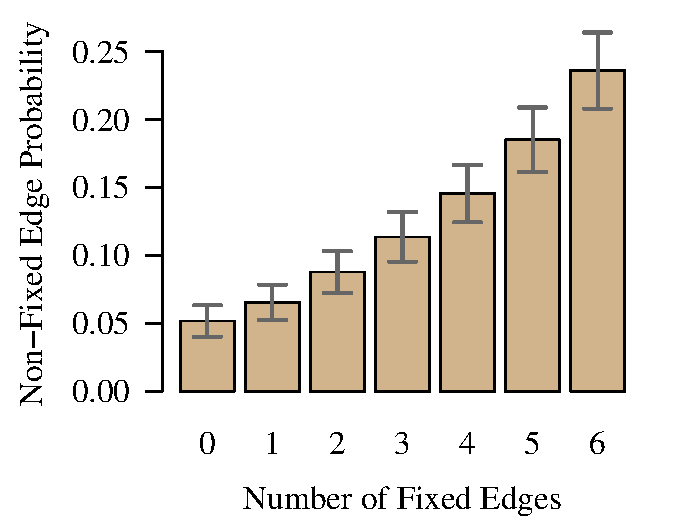
\includegraphics[scale=.85]{node_int.pdf}
\end{center}
\end{frame}


%%% Estimation, Challenges




\begin{frame}
\frametitle{Wrap-up}
\begin{itemize}
\item ERGM
\begin{itemize}
\item Test covariate effects
\item Test interdependence effects
\item Nothing like it in the literature
\end{itemize} ~\\~\\
\item Extensions
\begin{itemize}
\item Weighted Ties
\item Network time series
\item Bipartite networks
\end{itemize}
\end{itemize}
\end{frame}


\end{document}






\begin{frame}
\frametitle{ERGM Task List}


{\bf \Large What the Modeler Does:}
\begin{itemize}
\item Conceptually defines dependencies that should/might exist in the network.
\item Defines (selects) empirical measures of those dependencies. (i.e., $\bh(N)$)
\end{itemize} ~\\
{\bf \Large What ERGM Software Does:}
\begin{itemize}
\item Finds most likely set of $\bt$.
\item Simulates networks so you can check model fit.
\end{itemize}

\end{frame}


